%%%%%%%%%%%%%%%%%%%%%%%%%%%%%%%%%%%%%%%%%%%%%%%%%%%%%%%%%%%%%%%%%%%%%%%%%%%%%%%
% Chapter 3: Procedimiento experimental 
%%%%%%%%%%%%%%%%%%%%%%%%%%%%%%%%%%%%%%%%%%%%%%%%%%%%%%%%%%%%%%%%%%%%%%%%%%%%%%%

%++++++++++++++++++++++++++++++++++++++++++++++++++++++++++++++++++++++++++++++
\section{Descripci�n de los experimentos}
\label{3:sec:1}

  El experimento llevado a cabo en esta memoria ha consistido en la realizaci�n de varios c�digos en lenguaje $Python$. 
Los algoritmos implementados que solucionan dichos c�digos estiman la aproximaci�n $f(x) = sin(x)$ mediante el m�todo de Taylor, 
solicitando el grado del polinomio de Taylor, el punto central y el punto x donde se evalua dicho polinomio.
Para obtener varios valores del plinomio y as� poder comparar los datos obtenidos del error y el tiempo de CPU, se ha ejecutado el programa varias veces:
\begin{itemize}

\item Experimento 1:
 El grado del polinomio y el punto $c$ se dejaron fijos, variando solamente el punto $x$. 

\item Experimento 2: 
 El grado del polinomio tiene el mismo valor que en el experimento anterior, el valor de $x$ no var�a y el que lo hace es el punto $c$.

\item Experimento 3:
 El grado del polinomio es fijo con un valor mayor al de los anteriores experimentos. El punto $c$ es fijo y el punto $x$ se va modificiando.

\item Experimento 4:
 El grado del polinomio toma el valor de 100. El punto $c$ no cambia y el punto $x$ solo varia en las cantidad de cifras decimales. 

\end{itemize}
  

%++++++++++++++++++++++++++++++++++++++++++++++++++++++++++++++++++++++++++++++
\section{Descripci�n del material}
\label{3:sec:2}
  El material requerido para la realizaci�n del trabajo ha sido una computadora.
La que hemos utilizado para realizar estos experimentos tiene las siguientes caracteristicas: 
\begin{itemize}
 
  \item
   CPU type: Intel(R) Core(TM) i3-2328M CPU @ 2.50GHz
  \item
   vendor ID	GenuineIntel
  \item
    CPU speed	1200.000Hz
  \item
    cache size	2048 KB
  
\end{itemize}



%++++++++++++++++++++++++++++++++++++++++++++++++++++++++++++++++++++++++++++++
\section{Resultados obtenidos}
\label{3:sec:3}

%------------------------------------------------------------------------------
\begin{figure}[!th]
\begin{center}
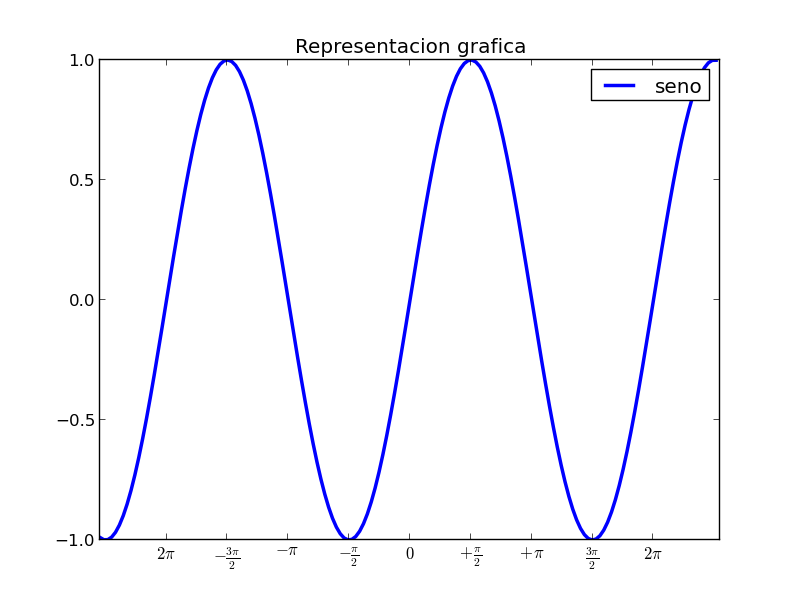
\includegraphics[width=0.75\textwidth]{images/grafico.eps}
\caption{Gr�fica de la funci�n original}
\label{fig:1}
\end{center}
\end{figure}
%------------------------------------------------------------------------------


%------------------------------------------------------------------------------
\begin{table}[!ht]
\begin{center}
\begin{tabular}{|l|c|c|c|c|c|}
\hline
Grado  & Punto c & Punto de Evaluacion & Aproximacion       & Error             & Tiempo CPU           \\ \hline
4      &   0.0   &    1                & 0.833333           & -0.833333         & 0.007406949996948242 \\ \hline
6      &   10    &    5                & 12.4605618963148   & -13.0045830072041 & 0.009202957153320312 \\ \hline
10     &   10    &    10               & -0.544021110889370 & 0                 & 0.010988950729370117  \\ \hline
\end{tabular}
\end{center}
\caption{Tabla de datos obtenidos experimentalmente}
\label{tab}
\end{table}

%------------------------------------------------------------------------------

%++++++++++++++++++++++++++++++++++++++++++++++++++++++++++++++++++++++++++++++
\section{An�lisis de los resultados}
\label{3:sec:4}
\begin{itemize}
\item Experimento 1:
 Polinomio de taylor de grado 4, punto $c=10.0$.
El punto de evaluci�n fue cambiando. A medida que se acercaba al punto $c$, el error fue disminuyendo. La diferencia del tiempo de CPU 
es m�nima. 
\item Experimento 2:
 Polinomio de Taylor de grado 4, punto $x=2.0$
El punto $c$ fue cambiando. Cuando el punto $c$ es 0, tanto el valor de aproximaci�n como el del error son iguales pero de signos diferentes. 
Si el valor otorgado a $c$ es negativo el error que se obtiene es mucho mas grande que si el valor de $c$ es positivo. 
\end{itemize}

